    
    
    
    

    

    \hypertarget{indexation-uxe9voluuxe9e}{%
\section{Indexation évoluée}\label{indexation-uxe9voluuxe9e}}

    \hypertarget{compluxe9ment---niveau-avancuxe9}{%
\subsection{Complément - niveau
avancé}\label{compluxe9ment---niveau-avancuxe9}}

    Nous allons maintenant voir qu'il est possible d'indexer un tableau
\texttt{numpy} avec, non pas des entiers ou des tuples comme on l'a vu
dans un complément précédent, mais aussi avec~d'autres types d'objets
qui permettent des manipulations très puissantes~:

\begin{itemize}
\tightlist
\item
  indexation par une liste~;
\item
  indexation par un tableau~;
\item
  indexation multiple (par un tuple)~;
\item
  indexation par un tableau de booléens.
\end{itemize}

    \begin{Verbatim}[commandchars=\\\{\},frame=single,framerule=0.3mm,rulecolor=\color{cellframecolor}]
{\color{incolor}In [{\color{incolor}1}]:} \PY{k+kn}{import} \PY{n+nn}{numpy} \PY{k}{as} \PY{n+nn}{np}
        \PY{k+kn}{import} \PY{n+nn}{matplotlib}\PY{n+nn}{.}\PY{n+nn}{pyplot} \PY{k}{as} \PY{n+nn}{plt}
        \PY{o}{\PYZpc{}}\PY{k}{matplotlib} inline
        \PY{n}{plt}\PY{o}{.}\PY{n}{ion}\PY{p}{(}\PY{p}{)}
\end{Verbatim}


    Pour illustrer ceci, on va réutiliser la fonction \texttt{background}
que l'on avait vue pour les indexations simples~:

    \begin{Verbatim}[commandchars=\\\{\},frame=single,framerule=0.3mm,rulecolor=\color{cellframecolor}]
{\color{incolor}In [{\color{incolor}2}]:} \PY{c+c1}{\PYZsh{} une fonction qui crée un tableau}
        \PY{c+c1}{\PYZsh{} tab[i, j] = i + 10 * j}
        \PY{k}{def} \PY{n+nf}{background}\PY{p}{(}\PY{n}{n}\PY{p}{)}\PY{p}{:}
            \PY{n}{i} \PY{o}{=} \PY{n}{np}\PY{o}{.}\PY{n}{arange}\PY{p}{(}\PY{n}{n}\PY{p}{)}
            \PY{n}{j} \PY{o}{=} \PY{n}{i}\PY{o}{.}\PY{n}{reshape}\PY{p}{(}\PY{p}{(}\PY{n}{n}\PY{p}{,} \PY{l+m+mi}{1}\PY{p}{)}\PY{p}{)}
            \PY{k}{return} \PY{n}{i} \PY{o}{+} \PY{l+m+mi}{10} \PY{o}{*} \PY{n}{j}
\end{Verbatim}


    \hypertarget{indexation-par-une-liste}{%
\subsubsection{Indexation par une
liste}\label{indexation-par-une-liste}}

    On peut indexer par une liste d'entiers, cela constitue une
généralisation des slices.

    \begin{Verbatim}[commandchars=\\\{\},frame=single,framerule=0.3mm,rulecolor=\color{cellframecolor}]
{\color{incolor}In [{\color{incolor}3}]:} \PY{n}{b} \PY{o}{=} \PY{n}{background}\PY{p}{(}\PY{l+m+mi}{6}\PY{p}{)}
        \PY{n+nb}{print}\PY{p}{(}\PY{n}{b}\PY{p}{)}
\end{Verbatim}


    \begin{Verbatim}[commandchars=\\\{\},frame=single,framerule=0.3mm,rulecolor=\color{cellframecolor}]
[[ 0  1  2  3  4  5]
 [10 11 12 13 14 15]
 [20 21 22 23 24 25]
 [30 31 32 33 34 35]
 [40 41 42 43 44 45]
 [50 51 52 53 54 55]]
\end{Verbatim}

    Si je veux référencer les lignes 1, 3 et 4, je ne peux pas utiliser un
slice~; mais je peux utiliser une liste à la place~:

    \begin{Verbatim}[commandchars=\\\{\},frame=single,framerule=0.3mm,rulecolor=\color{cellframecolor}]
{\color{incolor}In [{\color{incolor}4}]:} \PY{c+c1}{\PYZsh{} il faut lire ceci comme}
        \PY{c+c1}{\PYZsh{} j\PYZsq{}indexe b, avec comme indice la liste [1, 3, 4]}
        \PY{n}{b}\PY{p}{[}\PY{p}{[}\PY{l+m+mi}{1}\PY{p}{,} \PY{l+m+mi}{3}\PY{p}{,} \PY{l+m+mi}{4}\PY{p}{]}\PY{p}{]}
\end{Verbatim}


\begin{Verbatim}[commandchars=\\\{\},frame=single,framerule=0.3mm,rulecolor=\color{cellframecolor}]
{\color{outcolor}Out[{\color{outcolor}4}]:} array([[10, 11, 12, 13, 14, 15],
               [30, 31, 32, 33, 34, 35],
               [40, 41, 42, 43, 44, 45]])
\end{Verbatim}
            
    \begin{Verbatim}[commandchars=\\\{\},frame=single,framerule=0.3mm,rulecolor=\color{cellframecolor}]
{\color{incolor}In [{\color{incolor}5}]:} \PY{c+c1}{\PYZsh{} pareil pour les colonnes, en combinant avec un slice}
        \PY{n}{b}\PY{p}{[}\PY{p}{:}\PY{p}{,} \PY{p}{[}\PY{l+m+mi}{1}\PY{p}{,} \PY{l+m+mi}{3}\PY{p}{,} \PY{l+m+mi}{4}\PY{p}{]}\PY{p}{]}
\end{Verbatim}


\begin{Verbatim}[commandchars=\\\{\},frame=single,framerule=0.3mm,rulecolor=\color{cellframecolor}]
{\color{outcolor}Out[{\color{outcolor}5}]:} array([[ 1,  3,  4],
               [11, 13, 14],
               [21, 23, 24],
               [31, 33, 34],
               [41, 43, 44],
               [51, 53, 54]])
\end{Verbatim}
            
    \begin{Verbatim}[commandchars=\\\{\},frame=single,framerule=0.3mm,rulecolor=\color{cellframecolor}]
{\color{incolor}In [{\color{incolor}6}]:} \PY{c+c1}{\PYZsh{} et comme toujours on peut faire du broadcasting}
        \PY{n}{b}\PY{p}{[}\PY{p}{:}\PY{p}{,} \PY{p}{[}\PY{l+m+mi}{1}\PY{p}{,} \PY{l+m+mi}{3}\PY{p}{,} \PY{l+m+mi}{4}\PY{p}{]}\PY{p}{]} \PY{o}{=} \PY{n}{np}\PY{o}{.}\PY{n}{arange}\PY{p}{(}\PY{l+m+mi}{1000}\PY{p}{,} \PY{l+m+mi}{1006}\PY{p}{)}\PY{o}{.}\PY{n}{reshape}\PY{p}{(}\PY{p}{(}\PY{l+m+mi}{6}\PY{p}{,} \PY{l+m+mi}{1}\PY{p}{)}\PY{p}{)}
        \PY{n+nb}{print}\PY{p}{(}\PY{n}{b}\PY{p}{)}
\end{Verbatim}


    \begin{Verbatim}[commandchars=\\\{\},frame=single,framerule=0.3mm,rulecolor=\color{cellframecolor}]
[[   0 1000    2 1000 1000    5]
 [  10 1001   12 1001 1001   15]
 [  20 1002   22 1002 1002   25]
 [  30 1003   32 1003 1003   35]
 [  40 1004   42 1004 1004   45]
 [  50 1005   52 1005 1005   55]]
\end{Verbatim}

    \hypertarget{indexation-par-un-tableau}{%
\subsubsection{Indexation par un
tableau}\label{indexation-par-un-tableau}}

    On peut aussi indexer un tableau A \ldots{} par un tableau~! Pour que
cela ait un sens~:

\begin{itemize}
\tightlist
\item
  le tableau d'index doit contenir des entiers~;
\item
  ces derniers doivent être tous plus petits que la première dimension
  de A.
\end{itemize}

    \hypertarget{le-cas-simple-lentruxe9e-et-lindex-sont-de-dimension-1.}{%
\paragraph{Le cas simple~: l'entrée et l'index sont de dimension
1.}\label{le-cas-simple-lentruxe9e-et-lindex-sont-de-dimension-1.}}

    \begin{Verbatim}[commandchars=\\\{\},frame=single,framerule=0.3mm,rulecolor=\color{cellframecolor}]
{\color{incolor}In [{\color{incolor}7}]:} \PY{c+c1}{\PYZsh{} le tableau qu\PYZsq{}on va indexer}
        \PY{n}{cubes} \PY{o}{=} \PY{n}{np}\PY{o}{.}\PY{n}{arange}\PY{p}{(}\PY{l+m+mi}{10}\PY{p}{)} \PY{o}{*}\PY{o}{*} \PY{l+m+mi}{3}
        \PY{n+nb}{print}\PY{p}{(}\PY{n}{cubes}\PY{p}{)}
\end{Verbatim}


    \begin{Verbatim}[commandchars=\\\{\},frame=single,framerule=0.3mm,rulecolor=\color{cellframecolor}]
[  0   1   8  27  64 125 216 343 512 729]
\end{Verbatim}

    \begin{Verbatim}[commandchars=\\\{\},frame=single,framerule=0.3mm,rulecolor=\color{cellframecolor}]
{\color{incolor}In [{\color{incolor}8}]:} \PY{c+c1}{\PYZsh{} et un index qui est un tableau numpy}
        \PY{c+c1}{\PYZsh{} doit contenir des entiers entre 0 et 9}
        \PY{n}{tab} \PY{o}{=} \PY{n}{np}\PY{o}{.}\PY{n}{array}\PY{p}{(}\PY{p}{[}\PY{l+m+mi}{1}\PY{p}{,} \PY{l+m+mi}{7}\PY{p}{,} \PY{l+m+mi}{2}\PY{p}{]}\PY{p}{)}
        \PY{n+nb}{print}\PY{p}{(}\PY{n}{cubes}\PY{p}{[}\PY{n}{tab}\PY{p}{]}\PY{p}{)}
\end{Verbatim}


    \begin{Verbatim}[commandchars=\\\{\},frame=single,framerule=0.3mm,rulecolor=\color{cellframecolor}]
[  1 343   8]
\end{Verbatim}

    \begin{Verbatim}[commandchars=\\\{\},frame=single,framerule=0.3mm,rulecolor=\color{cellframecolor}]
{\color{incolor}In [{\color{incolor}9}]:} \PY{c+c1}{\PYZsh{} donne \PYZhy{} logiquement \PYZhy{} le même résultat que}
        \PY{c+c1}{\PYZsh{} si l\PYZsq{}index était une liste Python}
        \PY{n}{lis} \PY{o}{=} \PY{p}{[}\PY{l+m+mi}{1}\PY{p}{,} \PY{l+m+mi}{7}\PY{p}{,} \PY{l+m+mi}{2}\PY{p}{]}
        \PY{n+nb}{print}\PY{p}{(}\PY{n}{cubes}\PY{p}{[}\PY{n}{lis}\PY{p}{]}\PY{p}{)}
\end{Verbatim}


    \begin{Verbatim}[commandchars=\\\{\},frame=single,framerule=0.3mm,rulecolor=\color{cellframecolor}]
[  1 343   8]
\end{Verbatim}

    \hypertarget{de-maniuxe8re-guxe9nuxe9rale}{%
\paragraph{De manière générale}\label{de-maniuxe8re-guxe9nuxe9rale}}

    Dans le cas général, le résultat de \texttt{A{[}index{]}}~:

\begin{itemize}
\tightlist
\item
  a la même forme ``externe'' que \texttt{index}~;
\item
  où l'on a remplacé \texttt{i} par \texttt{A{[}i{]}}~;
\item
  qui peut donc être un tableau si \texttt{A} est de dimension
  \textgreater{} 1
\end{itemize}

    \begin{Verbatim}[commandchars=\\\{\},frame=single,framerule=0.3mm,rulecolor=\color{cellframecolor}]
{\color{incolor}In [{\color{incolor}10}]:} \PY{n}{A} \PY{o}{=} \PY{n}{np}\PY{o}{.}\PY{n}{array}\PY{p}{(}\PY{p}{[}\PY{p}{[}\PY{l+m+mi}{0}\PY{p}{,} \PY{l+s+s1}{\PYZsq{}}\PY{l+s+s1}{zero}\PY{l+s+s1}{\PYZsq{}}\PY{p}{]}\PY{p}{,} \PY{p}{[}\PY{l+m+mi}{1}\PY{p}{,} \PY{l+s+s1}{\PYZsq{}}\PY{l+s+s1}{un}\PY{l+s+s1}{\PYZsq{}}\PY{p}{]}\PY{p}{,} \PY{p}{[}\PY{l+m+mi}{2}\PY{p}{,} \PY{l+s+s1}{\PYZsq{}}\PY{l+s+s1}{deux}\PY{l+s+s1}{\PYZsq{}}\PY{p}{]}\PY{p}{,} \PY{p}{[}\PY{l+m+mi}{3}\PY{p}{,} \PY{l+s+s1}{\PYZsq{}}\PY{l+s+s1}{trois}\PY{l+s+s1}{\PYZsq{}}\PY{p}{]}\PY{p}{]}\PY{p}{)}
         \PY{n+nb}{print}\PY{p}{(}\PY{n}{A}\PY{p}{)}
\end{Verbatim}


    \begin{Verbatim}[commandchars=\\\{\},frame=single,framerule=0.3mm,rulecolor=\color{cellframecolor}]
[['0' 'zero']
 ['1' 'un']
 ['2' 'deux']
 ['3' 'trois']]
\end{Verbatim}

    \begin{Verbatim}[commandchars=\\\{\},frame=single,framerule=0.3mm,rulecolor=\color{cellframecolor}]
{\color{incolor}In [{\color{incolor}11}]:} \PY{n}{index} \PY{o}{=} \PY{n}{np}\PY{o}{.}\PY{n}{array}\PY{p}{(}\PY{p}{[}\PY{p}{[}\PY{l+m+mi}{1}\PY{p}{,} \PY{l+m+mi}{0}\PY{p}{,} \PY{l+m+mi}{2}\PY{p}{]}\PY{p}{,} \PY{p}{[}\PY{l+m+mi}{3}\PY{p}{,} \PY{l+m+mi}{2}\PY{p}{,} \PY{l+m+mi}{3}\PY{p}{]}\PY{p}{]}\PY{p}{)}
         \PY{n+nb}{print}\PY{p}{(}\PY{n}{index}\PY{p}{)}
\end{Verbatim}


    \begin{Verbatim}[commandchars=\\\{\},frame=single,framerule=0.3mm,rulecolor=\color{cellframecolor}]
[[1 0 2]
 [3 2 3]]
\end{Verbatim}

    \begin{figure}
\centering
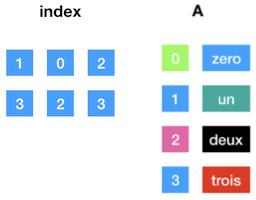
\includegraphics{media/index-parts.png}
\caption{parts}
\end{figure}

    \begin{Verbatim}[commandchars=\\\{\},frame=single,framerule=0.3mm,rulecolor=\color{cellframecolor}]
{\color{incolor}In [{\color{incolor}12}]:} \PY{n}{B} \PY{o}{=} \PY{n}{A}\PY{p}{[}\PY{n}{index}\PY{p}{]}
         \PY{n+nb}{print}\PY{p}{(}\PY{n}{B}\PY{p}{)}
\end{Verbatim}


    \begin{Verbatim}[commandchars=\\\{\},frame=single,framerule=0.3mm,rulecolor=\color{cellframecolor}]
[[['1' 'un']
  ['0' 'zero']
  ['2' 'deux']]

 [['3' 'trois']
  ['2' 'deux']
  ['3' 'trois']]]
\end{Verbatim}

    \begin{figure}
\centering
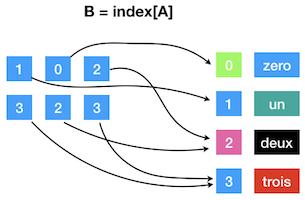
\includegraphics{media/index-result.png}
\caption{result}
\end{figure}

    \begin{Verbatim}[commandchars=\\\{\},frame=single,framerule=0.3mm,rulecolor=\color{cellframecolor}]
{\color{incolor}In [{\color{incolor}13}]:} \PY{n}{B}\PY{p}{[}\PY{l+m+mi}{1}\PY{p}{,} \PY{l+m+mi}{2}\PY{p}{,} \PY{l+m+mi}{1}\PY{p}{]}
\end{Verbatim}


\begin{Verbatim}[commandchars=\\\{\},frame=single,framerule=0.3mm,rulecolor=\color{cellframecolor}]
{\color{outcolor}Out[{\color{outcolor}13}]:} 'trois'
\end{Verbatim}
            
    \begin{figure}
\centering
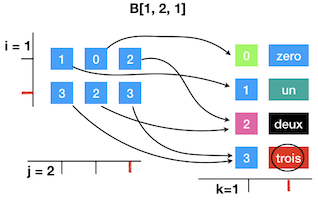
\includegraphics{media/index-detail.png}
\caption{result}
\end{figure}

    Et donc si~:

\begin{itemize}
\tightlist
\item
  \texttt{index} est de dimension \texttt{(i,\ j,\ k)}~;
\item
  \texttt{A} est de dimension \texttt{(a,\ b)}.
\end{itemize}

Alors :

\begin{itemize}
\tightlist
\item
  \texttt{A{[}index{]}} est de dimension \texttt{(i,\ j,\ k,\ b)}~;
\item
  il faut que les éléments dans \texttt{index} soient dans
  \texttt{{[}0\ ..\ a{[}}.
\end{itemize}

    Ce que l'on vérifie ici~:

    \begin{Verbatim}[commandchars=\\\{\},frame=single,framerule=0.3mm,rulecolor=\color{cellframecolor}]
{\color{incolor}In [{\color{incolor}14}]:} \PY{c+c1}{\PYZsh{} l\PYZsq{}entrée}
         \PY{n+nb}{print}\PY{p}{(}\PY{n}{A}\PY{o}{.}\PY{n}{shape}\PY{p}{)}
\end{Verbatim}


    \begin{Verbatim}[commandchars=\\\{\},frame=single,framerule=0.3mm,rulecolor=\color{cellframecolor}]
(4, 2)
\end{Verbatim}

    \begin{Verbatim}[commandchars=\\\{\},frame=single,framerule=0.3mm,rulecolor=\color{cellframecolor}]
{\color{incolor}In [{\color{incolor}15}]:} \PY{c+c1}{\PYZsh{} l\PYZsq{}index}
         \PY{n+nb}{print}\PY{p}{(}\PY{n}{index}\PY{o}{.}\PY{n}{shape}\PY{p}{)}
\end{Verbatim}


    \begin{Verbatim}[commandchars=\\\{\},frame=single,framerule=0.3mm,rulecolor=\color{cellframecolor}]
(2, 3)
\end{Verbatim}

    \begin{Verbatim}[commandchars=\\\{\},frame=single,framerule=0.3mm,rulecolor=\color{cellframecolor}]
{\color{incolor}In [{\color{incolor}16}]:} \PY{c+c1}{\PYZsh{} le résultat}
         \PY{n+nb}{print}\PY{p}{(}\PY{n}{A}\PY{p}{[}\PY{n}{index}\PY{p}{]}\PY{o}{.}\PY{n}{shape}\PY{p}{)}
\end{Verbatim}


    \begin{Verbatim}[commandchars=\\\{\},frame=single,framerule=0.3mm,rulecolor=\color{cellframecolor}]
(2, 3, 2)
\end{Verbatim}

    \hypertarget{cas-particulier-entruxe9e-de-dimension-1-index-de-dim.-1}{%
\paragraph{\texorpdfstring{Cas particulier~: entrée de dimension 1,
\texttt{index} de dim. \textgreater{}
1}{Cas particulier~: entrée de dimension 1, index de dim. \textgreater{} 1}}\label{cas-particulier-entruxe9e-de-dimension-1-index-de-dim.-1}}

Lorsque l'entrée \texttt{A} est de dimension 1, alors la sortie a
\textbf{exactement} la même forme que l'\texttt{index}.

C'est comme si \texttt{A} était une fonction que l'on applique aux
indices dans \texttt{index}.

    \begin{Verbatim}[commandchars=\\\{\},frame=single,framerule=0.3mm,rulecolor=\color{cellframecolor}]
{\color{incolor}In [{\color{incolor}17}]:} \PY{n+nb}{print}\PY{p}{(}\PY{n}{cubes}\PY{p}{)}
\end{Verbatim}


    \begin{Verbatim}[commandchars=\\\{\},frame=single,framerule=0.3mm,rulecolor=\color{cellframecolor}]
[  0   1   8  27  64 125 216 343 512 729]
\end{Verbatim}

    \begin{Verbatim}[commandchars=\\\{\},frame=single,framerule=0.3mm,rulecolor=\color{cellframecolor}]
{\color{incolor}In [{\color{incolor}18}]:} \PY{n}{i2} \PY{o}{=} \PY{n}{np}\PY{o}{.}\PY{n}{array}\PY{p}{(}\PY{p}{[}\PY{p}{[}\PY{l+m+mi}{2}\PY{p}{,} \PY{l+m+mi}{4}\PY{p}{]}\PY{p}{,} \PY{p}{[}\PY{l+m+mi}{8}\PY{p}{,} \PY{l+m+mi}{9}\PY{p}{]}\PY{p}{]}\PY{p}{)}
         \PY{n+nb}{print}\PY{p}{(}\PY{n}{i2}\PY{p}{)}
\end{Verbatim}


    \begin{Verbatim}[commandchars=\\\{\},frame=single,framerule=0.3mm,rulecolor=\color{cellframecolor}]
[[2 4]
 [8 9]]
\end{Verbatim}

    \begin{Verbatim}[commandchars=\\\{\},frame=single,framerule=0.3mm,rulecolor=\color{cellframecolor}]
{\color{incolor}In [{\color{incolor}19}]:} \PY{n+nb}{print}\PY{p}{(}\PY{n}{cubes}\PY{p}{[}\PY{n}{i2}\PY{p}{]}\PY{p}{)}
\end{Verbatim}


    \begin{Verbatim}[commandchars=\\\{\},frame=single,framerule=0.3mm,rulecolor=\color{cellframecolor}]
[[  8  64]
 [512 729]]
\end{Verbatim}

    \hypertarget{application-au-codage-des-couleurs-dans-une-image}{%
\paragraph{Application au codage des couleurs dans une
image}\label{application-au-codage-des-couleurs-dans-une-image}}

    \begin{Verbatim}[commandchars=\\\{\},frame=single,framerule=0.3mm,rulecolor=\color{cellframecolor}]
{\color{incolor}In [{\color{incolor}20}]:} \PY{c+c1}{\PYZsh{} je crée une image avec 6 valeurs disposées en diagonale}
         \PY{n}{N} \PY{o}{=} \PY{l+m+mi}{32}
         \PY{n}{colors} \PY{o}{=} \PY{l+m+mi}{6}
         
         \PY{n}{image} \PY{o}{=} \PY{n}{np}\PY{o}{.}\PY{n}{empty}\PY{p}{(}\PY{p}{(}\PY{n}{N}\PY{p}{,} \PY{n}{N}\PY{p}{)}\PY{p}{,} \PY{n}{dtype} \PY{o}{=} \PY{n}{np}\PY{o}{.}\PY{n}{int32}\PY{p}{)}
         \PY{k}{for} \PY{n}{i} \PY{o+ow}{in} \PY{n+nb}{range}\PY{p}{(}\PY{n}{N}\PY{p}{)}\PY{p}{:}
             \PY{k}{for} \PY{n}{j} \PY{o+ow}{in} \PY{n+nb}{range}\PY{p}{(}\PY{n}{N}\PY{p}{)}\PY{p}{:}
                \PY{n}{image}\PY{p}{[}\PY{n}{i}\PY{p}{,} \PY{n}{j}\PY{p}{]} \PY{o}{=} \PY{p}{(}\PY{n}{i}\PY{o}{+}\PY{n}{j}\PY{p}{)} \PY{o}{\PYZpc{}} \PY{n}{colors}
\end{Verbatim}


    \begin{Verbatim}[commandchars=\\\{\},frame=single,framerule=0.3mm,rulecolor=\color{cellframecolor}]
{\color{incolor}In [{\color{incolor}21}]:} \PY{n}{plt}\PY{o}{.}\PY{n}{imshow}\PY{p}{(}\PY{n}{image}\PY{p}{,} \PY{n}{cmap}\PY{o}{=}\PY{l+s+s1}{\PYZsq{}}\PY{l+s+s1}{gray}\PY{l+s+s1}{\PYZsq{}}\PY{p}{)}\PY{p}{;}
\end{Verbatim}


    \begin{center}
    \adjustimage{max size={0.9\linewidth}{0.9\paperheight}}{w7-s05-c5-indexation-evoluee_files/w7-s05-c5-indexation-evoluee_40_0.png}
    \end{center}
    { \hspace*{\fill} \\}
    
    Les couleurs ne sont pas significatives, ce sont des valeurs entières
dans \texttt{range(colors)}. On voudrait pouvoir choisir la vraie
couleur correspondant à chaque valeur. Pour cela on peut utiliser une
simple indexation par tableau~:

    \begin{Verbatim}[commandchars=\\\{\},frame=single,framerule=0.3mm,rulecolor=\color{cellframecolor}]
{\color{incolor}In [{\color{incolor}22}]:} \PY{c+c1}{\PYZsh{} une palette de couleurs}
         \PY{n}{palette} \PY{o}{=} \PY{n}{np}\PY{o}{.}\PY{n}{array}\PY{p}{(}\PY{p}{[}
           \PY{p}{[}\PY{l+m+mi}{255}\PY{p}{,} \PY{l+m+mi}{255}\PY{p}{,} \PY{l+m+mi}{255}\PY{p}{]}\PY{p}{,} \PY{c+c1}{\PYZsh{} 0 \PYZhy{}\PYZgt{} blanc}
           \PY{p}{[}\PY{l+m+mi}{255}\PY{p}{,} \PY{l+m+mi}{0}\PY{p}{,} \PY{l+m+mi}{0}\PY{p}{]}\PY{p}{,}     \PY{c+c1}{\PYZsh{} 1 \PYZhy{}\PYZgt{} rouge}
           \PY{p}{[}\PY{l+m+mi}{0}\PY{p}{,} \PY{l+m+mi}{255}\PY{p}{,} \PY{l+m+mi}{0}\PY{p}{]}\PY{p}{,}     \PY{c+c1}{\PYZsh{} 2 \PYZhy{}\PYZgt{} vert}
           \PY{p}{[}\PY{l+m+mi}{0}\PY{p}{,} \PY{l+m+mi}{0}\PY{p}{,} \PY{l+m+mi}{255}\PY{p}{]}\PY{p}{,}     \PY{c+c1}{\PYZsh{} 3 \PYZhy{}\PYZgt{} bleu}
           \PY{p}{[}\PY{l+m+mi}{0}\PY{p}{,} \PY{l+m+mi}{255}\PY{p}{,} \PY{l+m+mi}{255}\PY{p}{]}\PY{p}{,}   \PY{c+c1}{\PYZsh{} 4 \PYZhy{}\PYZgt{} cyan}
           \PY{p}{[}\PY{l+m+mi}{255}\PY{p}{,} \PY{l+m+mi}{255}\PY{p}{,} \PY{l+m+mi}{0}\PY{p}{]}\PY{p}{,}   \PY{c+c1}{\PYZsh{} 5 \PYZhy{}\PYZgt{} magenta}
          \PY{p}{]}\PY{p}{,} \PY{n}{dtype}\PY{o}{=}\PY{n}{np}\PY{o}{.}\PY{n}{uint8}\PY{p}{)}
\end{Verbatim}


    \begin{Verbatim}[commandchars=\\\{\},frame=single,framerule=0.3mm,rulecolor=\color{cellframecolor}]
{\color{incolor}In [{\color{incolor}23}]:} \PY{n}{plt}\PY{o}{.}\PY{n}{imshow}\PY{p}{(}\PY{n}{palette}\PY{p}{[}\PY{n}{image}\PY{p}{]}\PY{p}{)}\PY{p}{;}
\end{Verbatim}


    \begin{center}
    \adjustimage{max size={0.9\linewidth}{0.9\paperheight}}{w7-s05-c5-indexation-evoluee_files/w7-s05-c5-indexation-evoluee_43_0.png}
    \end{center}
    { \hspace*{\fill} \\}
    
    Remarquez que la forme générale n'a pas changé, mais le résultat de
l'indexation a une dimension supplémentaire de 3 couleurs~:

    \begin{Verbatim}[commandchars=\\\{\},frame=single,framerule=0.3mm,rulecolor=\color{cellframecolor}]
{\color{incolor}In [{\color{incolor}24}]:} \PY{n}{image}\PY{o}{.}\PY{n}{shape}
\end{Verbatim}


\begin{Verbatim}[commandchars=\\\{\},frame=single,framerule=0.3mm,rulecolor=\color{cellframecolor}]
{\color{outcolor}Out[{\color{outcolor}24}]:} (32, 32)
\end{Verbatim}
            
    \begin{Verbatim}[commandchars=\\\{\},frame=single,framerule=0.3mm,rulecolor=\color{cellframecolor}]
{\color{incolor}In [{\color{incolor}25}]:} \PY{n}{palette}\PY{p}{[}\PY{n}{image}\PY{p}{]}\PY{o}{.}\PY{n}{shape}
\end{Verbatim}


\begin{Verbatim}[commandchars=\\\{\},frame=single,framerule=0.3mm,rulecolor=\color{cellframecolor}]
{\color{outcolor}Out[{\color{outcolor}25}]:} (32, 32, 3)
\end{Verbatim}
            
    \hypertarget{indexation-multiple-par-tuple}{%
\subsubsection{Indexation multiple (par
tuple)}\label{indexation-multiple-par-tuple}}

    Une fois que vous avez compris ce mécanisme d'indexation par un tableau,
on peut encore généraliser pour définir une indexation par deux (ou
plus) tableaux de formes identiques.

    Ainsi, lorsque \texttt{index1} et \texttt{index2} ont la même forme~:

\begin{itemize}
\tightlist
\item
  on peut écrire \texttt{A{[}index1,\ index2{]}}
\item
  qui a la même forme externe que les \texttt{index}
\item
  où on a remplacé \texttt{i,\ j} par \texttt{A{[}i{]}{[}j{]}}
\item
  qui peut donc être un tableau si \texttt{A} est de dimension
  \textgreater{} 2.
\end{itemize}

    \begin{Verbatim}[commandchars=\\\{\},frame=single,framerule=0.3mm,rulecolor=\color{cellframecolor}]
{\color{incolor}In [{\color{incolor}26}]:} \PY{c+c1}{\PYZsh{} un tableau à indexer}
         \PY{n}{ix}\PY{p}{,} \PY{n}{iy} \PY{o}{=} \PY{n}{np}\PY{o}{.}\PY{n}{indices}\PY{p}{(}\PY{p}{(}\PY{l+m+mi}{4}\PY{p}{,} \PY{l+m+mi}{3}\PY{p}{)}\PY{p}{)}
         \PY{n}{A} \PY{o}{=} \PY{l+m+mi}{10} \PY{o}{*} \PY{n}{ix} \PY{o}{+} \PY{n}{iy}
         \PY{n+nb}{print}\PY{p}{(}\PY{n}{A}\PY{p}{)}
\end{Verbatim}


    \begin{Verbatim}[commandchars=\\\{\},frame=single,framerule=0.3mm,rulecolor=\color{cellframecolor}]
[[ 0  1  2]
 [10 11 12]
 [20 21 22]
 [30 31 32]]
\end{Verbatim}

    \begin{Verbatim}[commandchars=\\\{\},frame=single,framerule=0.3mm,rulecolor=\color{cellframecolor}]
{\color{incolor}In [{\color{incolor}27}]:} \PY{c+c1}{\PYZsh{} les deux tableaux d\PYZsq{}indices sont carrés 2x2}
         \PY{n}{index1} \PY{o}{=} \PY{p}{[}\PY{p}{[}\PY{l+m+mi}{3}\PY{p}{,} \PY{l+m+mi}{2}\PY{p}{]}\PY{p}{,} \PY{p}{[}\PY{l+m+mi}{0}\PY{p}{,} \PY{l+m+mi}{1} \PY{p}{]}\PY{p}{]}  \PY{c+c1}{\PYZsh{} doivent être \PYZlt{} 4}
         \PY{n}{index2} \PY{o}{=} \PY{p}{[}\PY{p}{[}\PY{l+m+mi}{2}\PY{p}{,} \PY{l+m+mi}{0}\PY{p}{]}\PY{p}{,} \PY{p}{[}\PY{l+m+mi}{0}\PY{p}{,} \PY{l+m+mi}{2} \PY{p}{]}\PY{p}{]}  \PY{c+c1}{\PYZsh{} doivent être \PYZlt{} 3}
         \PY{c+c1}{\PYZsh{} le résultat est donc carré 2x2}
         \PY{n+nb}{print}\PY{p}{(}\PY{n}{A}\PY{p}{[}\PY{n}{index1}\PY{p}{,} \PY{n}{index2}\PY{p}{]}\PY{p}{)}
\end{Verbatim}


    \begin{Verbatim}[commandchars=\\\{\},frame=single,framerule=0.3mm,rulecolor=\color{cellframecolor}]
[[32 20]
 [ 0 12]]
\end{Verbatim}

    Et donc si~:

\begin{itemize}
\tightlist
\item
  \texttt{index1} et \texttt{index2} sont de dimension
  \texttt{(i,\ j,\ k)}
\item
  et \texttt{A} est de dimension \texttt{(a,\ b,\ c)}
\end{itemize}

Alors~:

\begin{itemize}
\tightlist
\item
  le résultat est de dimension \texttt{(i,\ j,\ k,\ c)}
\item
  il faut alors que les éléments de \texttt{index1} soient dans
  \texttt{{[}0\ ..\ a{[}}
\item
  et les éléments de \texttt{index2} dans \texttt{{[}0\ ..\ b{[}}
\end{itemize}

    \hypertarget{application-uxe0-la-recherche-de-maxima}{%
\paragraph{Application à la recherche de
maxima}\label{application-uxe0-la-recherche-de-maxima}}

    Imaginons que vous avez des mesures pour plusieurs instants~:

    \begin{Verbatim}[commandchars=\\\{\},frame=single,framerule=0.3mm,rulecolor=\color{cellframecolor}]
{\color{incolor}In [{\color{incolor}28}]:} \PY{n}{times} \PY{o}{=} \PY{n}{np}\PY{o}{.}\PY{n}{linspace}\PY{p}{(}\PY{l+m+mi}{1000}\PY{p}{,} \PY{l+m+mi}{5000}\PY{p}{,} \PY{n}{num}\PY{o}{=}\PY{l+m+mi}{5}\PY{p}{,} \PY{n}{dtype}\PY{o}{=}\PY{n+nb}{int}\PY{p}{)}
         \PY{n+nb}{print}\PY{p}{(}\PY{n}{times}\PY{p}{)}
\end{Verbatim}


    \begin{Verbatim}[commandchars=\\\{\},frame=single,framerule=0.3mm,rulecolor=\color{cellframecolor}]
[1000 2000 3000 4000 5000]
\end{Verbatim}

    \begin{Verbatim}[commandchars=\\\{\},frame=single,framerule=0.3mm,rulecolor=\color{cellframecolor}]
{\color{incolor}In [{\color{incolor}29}]:} \PY{c+c1}{\PYZsh{} on aurait 3 mesures à chaque instant}
         \PY{n}{series} \PY{o}{=} \PY{n}{np}\PY{o}{.}\PY{n}{array}\PY{p}{(}\PY{p}{[}
             \PY{p}{[}\PY{l+m+mi}{10}\PY{p}{,} \PY{l+m+mi}{25}\PY{p}{,} \PY{l+m+mi}{32}\PY{p}{,} \PY{l+m+mi}{23}\PY{p}{,} \PY{l+m+mi}{12}\PY{p}{]}\PY{p}{,}
             \PY{p}{[}\PY{l+m+mi}{12}\PY{p}{,} \PY{l+m+mi}{8}\PY{p}{,} \PY{l+m+mi}{4}\PY{p}{,} \PY{l+m+mi}{10}\PY{p}{,} \PY{l+m+mi}{7}\PY{p}{]}\PY{p}{,}
             \PY{p}{[}\PY{l+m+mi}{100}\PY{p}{,} \PY{l+m+mi}{80}\PY{p}{,} \PY{l+m+mi}{90}\PY{p}{,} \PY{l+m+mi}{110}\PY{p}{,} \PY{l+m+mi}{120}\PY{p}{]}\PY{p}{]}\PY{p}{)}
         \PY{n+nb}{print}\PY{p}{(}\PY{n}{series}\PY{p}{)}
\end{Verbatim}


    \begin{Verbatim}[commandchars=\\\{\},frame=single,framerule=0.3mm,rulecolor=\color{cellframecolor}]
[[ 10  25  32  23  12]
 [ 12   8   4  10   7]
 [100  80  90 110 120]]
\end{Verbatim}

    Avec la fonction \texttt{np.maxargs} on peut retrouver les indices des
points maxima dans \texttt{series}~:

    \begin{Verbatim}[commandchars=\\\{\},frame=single,framerule=0.3mm,rulecolor=\color{cellframecolor}]
{\color{incolor}In [{\color{incolor}30}]:} \PY{n}{max\PYZus{}indices} \PY{o}{=} \PY{n}{np}\PY{o}{.}\PY{n}{argmax}\PY{p}{(}\PY{n}{series}\PY{p}{,} \PY{n}{axis}\PY{o}{=}\PY{l+m+mi}{1}\PY{p}{)}
         \PY{n+nb}{print}\PY{p}{(}\PY{n}{max\PYZus{}indices}\PY{p}{)}
\end{Verbatim}


    \begin{Verbatim}[commandchars=\\\{\},frame=single,framerule=0.3mm,rulecolor=\color{cellframecolor}]
[2 0 4]
\end{Verbatim}

    Pour trouver les maxima en question, on peut faire~:

    \begin{Verbatim}[commandchars=\\\{\},frame=single,framerule=0.3mm,rulecolor=\color{cellframecolor}]
{\color{incolor}In [{\color{incolor}31}]:} \PY{c+c1}{\PYZsh{} les trois maxima, un par serie}
         \PY{n}{maxima} \PY{o}{=} \PY{n}{series}\PY{p}{[} \PY{n+nb}{range}\PY{p}{(}\PY{n}{series}\PY{o}{.}\PY{n}{shape}\PY{p}{[}\PY{l+m+mi}{0}\PY{p}{]}\PY{p}{)}\PY{p}{,} \PY{n}{max\PYZus{}indices} \PY{p}{]}
         \PY{n+nb}{print}\PY{p}{(}\PY{n}{maxima}\PY{p}{)}
\end{Verbatim}


    \begin{Verbatim}[commandchars=\\\{\},frame=single,framerule=0.3mm,rulecolor=\color{cellframecolor}]
[ 32  12 120]
\end{Verbatim}

    \begin{Verbatim}[commandchars=\\\{\},frame=single,framerule=0.3mm,rulecolor=\color{cellframecolor}]
{\color{incolor}In [{\color{incolor}32}]:} \PY{c+c1}{\PYZsh{} et ils correspondent à ces instants\PYZhy{}ci}
         \PY{n}{times}\PY{p}{[}\PY{n}{max\PYZus{}indices}\PY{p}{]}
\end{Verbatim}


\begin{Verbatim}[commandchars=\\\{\},frame=single,framerule=0.3mm,rulecolor=\color{cellframecolor}]
{\color{outcolor}Out[{\color{outcolor}32}]:} array([3000, 1000, 5000])
\end{Verbatim}
            
    \hypertarget{indexation-par-un-tableau-de-booluxe9ens}{%
\subsubsection{Indexation par un tableau de
booléens}\label{indexation-par-un-tableau-de-booluxe9ens}}

    Une forme un peu spéciale d'indexation consiste à utiliser un tableau de
booléens, qui agit comme un masque~:

    \begin{Verbatim}[commandchars=\\\{\},frame=single,framerule=0.3mm,rulecolor=\color{cellframecolor}]
{\color{incolor}In [{\color{incolor}33}]:} \PY{n}{suite} \PY{o}{=} \PY{n}{np}\PY{o}{.}\PY{n}{array}\PY{p}{(}\PY{p}{[}\PY{l+m+mi}{1}\PY{p}{,} \PY{l+m+mi}{2}\PY{p}{,} \PY{l+m+mi}{3}\PY{p}{,} \PY{l+m+mi}{4}\PY{p}{,} \PY{l+m+mi}{5}\PY{p}{,} \PY{l+m+mi}{4}\PY{p}{,} \PY{l+m+mi}{3}\PY{p}{,} \PY{l+m+mi}{2}\PY{p}{,} \PY{l+m+mi}{1}\PY{p}{]}\PY{p}{)}
\end{Verbatim}


    Je veux filtrer ce tableau et ne garder que les valeurs \textless{} 4~:

    \begin{Verbatim}[commandchars=\\\{\},frame=single,framerule=0.3mm,rulecolor=\color{cellframecolor}]
{\color{incolor}In [{\color{incolor}34}]:} \PY{c+c1}{\PYZsh{} je construis un masque}
         \PY{n}{hauts} \PY{o}{=} \PY{n}{suite} \PY{o}{\PYZgt{}}\PY{o}{=} \PY{l+m+mi}{4}
         \PY{n+nb}{print}\PY{p}{(}\PY{n}{hauts}\PY{p}{)}
\end{Verbatim}


    \begin{Verbatim}[commandchars=\\\{\},frame=single,framerule=0.3mm,rulecolor=\color{cellframecolor}]
[False False False  True  True  True False False False]
\end{Verbatim}

    \begin{Verbatim}[commandchars=\\\{\},frame=single,framerule=0.3mm,rulecolor=\color{cellframecolor}]
{\color{incolor}In [{\color{incolor}35}]:} \PY{c+c1}{\PYZsh{} je peux utiliser ce masque pour calculer les indices qui sont vrais}
         \PY{n}{suite}\PY{p}{[}\PY{n}{hauts}\PY{p}{]}
\end{Verbatim}


\begin{Verbatim}[commandchars=\\\{\},frame=single,framerule=0.3mm,rulecolor=\color{cellframecolor}]
{\color{outcolor}Out[{\color{outcolor}35}]:} array([4, 5, 4])
\end{Verbatim}
            
    \begin{Verbatim}[commandchars=\\\{\},frame=single,framerule=0.3mm,rulecolor=\color{cellframecolor}]
{\color{incolor}In [{\color{incolor}36}]:} \PY{c+c1}{\PYZsh{} et utiliser maintenant ceci par un index de tableau}
         \PY{c+c1}{\PYZsh{} par exemple pour annuler ces valeurs}
         \PY{n}{suite}\PY{p}{[}\PY{n}{hauts}\PY{p}{]} \PY{o}{=} \PY{l+m+mi}{0}
         \PY{n+nb}{print}\PY{p}{(}\PY{n}{suite}\PY{p}{)}
\end{Verbatim}


    \begin{Verbatim}[commandchars=\\\{\},frame=single,framerule=0.3mm,rulecolor=\color{cellframecolor}]
[1 2 3 0 0 0 3 2 1]
\end{Verbatim}


    % Add a bibliography block to the postdoc
    
    
    
